\documentclass{SeminarV2}
\usepackage{graphicx}
\usepackage[utf8]{inputenc}
\usepackage{amssymb,amsmath,array}

%***********************************************************************
% !!!! IMPORTANT NOTICE ON TEXT MARGINS !!!!!
%***********************************************************************
%
% Please avoid using DVI2PDF or PS2PDF converters: some undesired
% shifting/scaling may occur when using these programs
% It is strongly recommended to use the DVIPS converters.
%
% Check that you have set the paper size to A4 (and NOT to letter) in your
% dvi2ps converter, in Adobe Acrobat if you use it, and in any printer driver
% that you could use.  You also have to disable the 'scale to fit paper' option
% of your printer driver.
%
% In any case, please check carefully that the final size of the top and
% bottom margins is 5.2 cm and of the left and right margins is 4.4 cm.
% It is your responsibility to verify this important requirement.  
% If these margin requirements and not fulfilled at the end of your file generation process, please use the following commands to correct them.  Otherwise, please do not modify these commands.
%
\voffset 0 cm \hoffset 0 cm \addtolength{\textwidth}{0cm}
\addtolength{\textheight}{0cm}\addtolength{\leftmargin}{0cm}

%***********************************************************************
% !!!! USE OF THE SeminarV2 LaTeX STYLE FILE !!!!!
%***********************************************************************
%
% Some commands are inserted in the following .tex example file.  Therefore to
% set up your Seminar submission, please use this file and modify it to insert
% your text, rather than staring from a blank .tex file.  In this way, you will
% have the commands inserted in the right place.

% Edited by Martin Bogdan.

\begin{document}
%style file for Seminar manuscripts
\title{Simulation der Histonmodifikation}

%***********************************************************************
% AUTHORS INFORMATION AREA
%***********************************************************************
\author{Max Hild
% DO NOT MODIFY THE FOLLOWING '\vspace' ARGUMENT
\vspace{.3cm}\\
%
% Addresses and institutions (remove "1- " in case of a single institution)
\emph{Abgegeben bei: Dr. J\"{o}rg Galle, Prof. Dr. Markus Scholz}
% Remove the next three lines in case of a single institution
\vspace{.1cm}\\
Universit\"{a}t Leipzig, Institut f\"{u}r medizinische Informatik, Statistik und Epidemiologie\\
Neues Augusteum, Augustuspl. 10, 04109 Leipzig - Germany
}


%***********************************************************************
% END OF AUTHORS INFORMATION AREA
%***********************************************************************

\maketitle

\begin{abstract}
  \sloppy
  GWAS (Genome-Wide Association Studies) sind eine weit verbreitete Methode
  zur Identifizierung von genetischen Varianten, die mit komplexen Erkrankungen assoziiert sein k\"{o}nnten.
  Einer der treibenden Faktoren der Weiterentwicklung der Forschung zum menschlichen Genom
  war in den letzten Jahren jedoch eine Abkehr von der klassischen Sichtweise, dass die
  gesamte Heritabilit\"{a}t von Ph\"{a}notypen lediglich durch die genetische Kodierung
  erkl\"{a}rt werden kann. In GWAS erreichten die relevanten Ma{\ss}zahlen f\"{u}r die Heritabilit\"{a}t
  wiederholt lediglich kleine Werte. \cite{mcclellan-2010}
    
  Hier zeigte sich, dass weitere Forschungszweige wie die Transkriptionsanalyse
  sowie die Epigenetik notwendig sind, um die fehlende Heritabilit\"{a}t der Ph\"{a}notypen zu erkl\"{a}ren. 
  Epigenetische Mechanismen wie DNA-Methylierung und Histonmodifikationen spielen eine entscheidende 
  Rolle bei der Regulation der Genexpression und k\"{o}nnten somit einen Teil der fehlenden Heritabilit\"{a}t 
  erkl\"{a}ren. Diese Mechanismen sind dynamisch und k\"{o}nnen durch Umweltfaktoren beeinflusst werden, 
  was sie zu einem spannenden Forschungsfeld macht.
  \end{abstract}
  

\section{Einleitung}
Die Heritabilit\"{a}t von Ph\"{a}notypen besser zu erforschen l\"{a}sst Forscherinnen und Forscher leichter
nachvollziehen, wie die genetische Information kodiert ist.
Prohaska et al. argumentieren, dass die Bedeutung des regulatorischen Systems der Epigenetik f\"{u}r die Vererbung gro{\ss} ist.
Sie skizzieren ein komputationales Modell, dass Reader und Writer Proteine verwendet, die durch eine zugrundeliegende Regulationsfunktion die DNA Replikation sowie Transkription steuern.
Dieses System wird in Prohaska et al. mit einem deterministischen System beschrieben, das die Dynamik der epigenetischen Zust\"{a}nde an CpG-Stellen in einem Genom simuliert.
Das regulatorische System der Epigenetik wird als ein Schlüssel zur erkennung der fehlenden Heritabilität gesehen.
Diese anerkannte Theorie wird durch Evidenz unterstützt. Jedoch ist es noch ein Forschungsgegenstand, wie genau die komplexeren Systeme, die bei Eukaryoten zu finden sind, gesteuert werden. \cite{prohaska-2010}
Auch aus der Sicht von Bannister {\&} Kouzarides spielen Histonmodifikationen eine zentrale Rolle im epigenetischen Code. 
Sie beschreiben die verschiedenen Writer, Eraser und Reader von Histonmarken und deren Einfluss auf Transkription, DNA-Reparatur und Chromosomenkondensation \cite{bannister-2011}.  
Transgenerationale Epigenetikstudien zeigen zudem, dass bestimmte epigenetische Markierungen selbst \"{u}ber mehrere Generationen hinweg erhalten bleiben k\"{o}nnen und so zur fehlenden Heritabilit\"{a}t beitragen \cite{tollefsbol-2014}.
Diese Forschung deckt sich mit der Einschätzung von McClellan et al.
die in ihrer Arbeit ein Pl\"{a}doyer f\"{u}r die Forschung
nach der fehlenden Heritabilit\"{a}t halten.
\begin{quote}
  \sloppy
  Eine der gr\"{o}{\ss}en Hoffnungen an die GWAS war, dass man - 
  genauso wie eine Vielzahl von mendelschen Erkrankungen auf DNA-Ebene 
  eingegrenzt und das beteiligte Gen samt den Mutationen identifiziert werden konnte - 
  einfach von Einzelgen-Erkrankungen auf komplexe multigenetische Erkrankungen schlie{\ss}en k\"{o}nnte. 
  Das ist jedoch nicht eingetreten. Bef\"{u}rworter werden argumentieren, dass es funktioniert hat 
  und dass allerlei faszinierende Gene identifiziert wurden, die beispielsweise eine Pr\"{a}disposition 
  zu oder einen Schutz vor Diabetes oder Brustkrebs verleihen, aber die Tatsache bleibt, dass der Gro{\ss}teil 
  der Erblichkeit in diesen Erkrankungen nicht den durch GWAS identifizierten Loci zugeschrieben werden 
  kann, was eindeutig zeigt, dass dies nicht die universelle L\"{o}sung sein wird.
  \cite{mcclellan-2010}
\end{quote}
Zu verstehen, wie die Modifikation der Histone und DNA-Methylierung funktioniert, ist nach heutiger Sicht ein wesentlicher Schritt, um die L\"{u}cke in unserem Verst\"{a}ndnis der Heritabilit\"{a}t zu schlie{\ss}en.

\section{Methoden}

Zentraler Bestandteil dieser Arbeit ist der Vergleich eines stochastischen Modells, welches auf Basis von Markov Ketten mittels \"{U}bergangswahrscheinlichkeiten die Histonmodifikation simuliert, mit einem Modell welches auf der Forschung von
Prohaska et al. basiert.
Das Modell von Prohaska et al. beschreibt die Histonmodifikation als ein deterministisches System.
Es definiert jeden Nukleosom‑Knoten durch zwei Flags für Acetylation (H3K27ac) und Methylation (H3K9me3) sowie einen Aktivitätsindikator. In jedem Zeitschritt werden alle Nukleosomen gleichzeitig nach folgenden Regeln aktualisiert: Ein Nukleosom erwirbt Acetylation, falls sein linker Nachbar bereits acetylierte Kennzeichnungen besitzt, andernfalls erhält es Methylation, falls sein rechter Nachbar methy­liert ist. Diese strikt logischen Booleschen Operationen werden in der Methode \texttt{applyDeterministicProhaskaRules()} umgesetzt.
Diese Zustände entscheiden darüber, ob die DNA an dieser Stelle für die Transkription verwendet werden kann.
Methylierte Stellen sind gebunden, während 
CpG-Stellen sind spezifische DNA-Sequenzen, die eine hohe Dichte an Cytosin- und Guanin-Basenpaaren aufweisen. 
Diese Stellen können durch ihre chemische Zusammensetzung

\subsection{Markov-Modell (stochastischer Ansatz)}
Zur Modellierung der DNA-Histonmodifikation wurde eine C++ Implementierung entwickelt, die auf dem Modell von Prohaska et al. basiert. Das Modell simuliert die dynamischen Ver\"{a}nderungen der epigenetischen Zust\"{a}nde an CpG-Stellen \"{u}ber die Zeit. Jede CpG-Stelle kann einen von f\"{u}nf m\"{o}glichen Zust\"{a}nden annehmen:
Das stochastische Modell basiert auf einem Markov-Prozess, der Übergänge zwischen fünf möglichen Zuständen an jeder CpG-Stelle beschreibt: Unmethyliert (U), Methyliert (M), Histon-modifiziert (H), Vollständig modifiziert (F, sowohl methyliert als auch Histon-modifiziert) und Komplex-gebunden (C). Diese Übergänge werden mit Wahrscheinlichkeiten gesteuert, die auf empirischen Daten beruhen (z.B. Fu et al., 2010). Jeder Zeitschritt besteht darin, für jede CpG-Stelle den nächsten Zustand basierend auf den definierten Übergangswahrscheinlichkeiten zufällig zu wählen. Zusätzlich zur zufälligen Auswahl wird im Modell eine deterministische Komponente integriert, indem die Prohaska-Regeln vor jedem stochastischen Schritt angewendet werden. Dadurch entsteht ein hybrider Ansatz, der sowohl deterministische Nachbarschaftsregeln als auch stochastische Veränderungen abbildet und somit biologisch realistischer sein könnte.

Die \"{U}berg\"{a}nge zwischen diesen Zust\"{a}nden 
werden durch ein stochastisches Modell gesteuert, das die 
biologischen Prozesse der Modifikation und Demodifikation nachbildet. 
Die Implementierung verwendet einen Markov-Prozess, bei dem die 
\"{u}bergangswahrscheinlichkeiten von den aktuellen Zust\"{a}nden benachbarter CpG-Stellen abh\"{a}ngen.

\subsection{Visualisierung}

Die Visualisierung besteht aus zwei Teilen: Die Heatmap wurde verwendet, um den Zustand jeder einzelnen CpG-Stelle \"{u}ber die Zeit darzustellen.
Das Liniendiagramm zeigt die H\"{a}ufigkeit jedes Zustands \"{u}ber die Zeit.
Die Simulation wird in Zeitschritten von 1 Zeiteinheit durchgef\"{u}hrt, wobei die \"{U}bergangswahrscheinlichkeiten f\"{u}r jeden Zustand und jede Nachbarschaftskonfiguration in einer Matrix gespeichert sind. Die Simulation wird f\"{u}r eine bestimmte Anzahl von Iterationen durchgef\"{u}hrt, um die zeitliche Entwicklung der CpG-Stellen zu beobachten.

\textbf{Technische Details:}
Die \texttt{CpGSite}-Klasse speichert den aktuellen Zustand als Enum und stellt Methoden zum Setzen und Abfragen des Zustands bereit.
Die \texttt{Genome}-Klasse verwaltet eine Liste von \texttt{CpGSite}-Objekten und erm\"{o}glicht den Zugriff auf benachbarte Stellen, was f\"{u}r die konditionalen \"{U}berg\"{a}nge notwendig ist.
In der \texttt{Simulator}-Klasse wird die Simulationslogik implementiert. Sie verwendet einen Zufallszahlengenerator, um stochastische \"{U}berg\"{a}nge gem\"{a}\ss den spezifizierten Wahrscheinlichkeiten durchzuf\"{u}hren. Die \"{U}bergangswahrscheinlichkeiten sind in einer Matrix abgelegt, die f\"{u}r jeden Zustand und jede Nachbarschaftskonfiguration die jeweilige Wahrscheinlichkeit enth\"{a}lt.
Die Ergebnisse werden nach jedem Zeitschritt in eine CSV-Datei geschrieben. Diese Datei enth\"{a}lt sowohl den Zustand jeder CpG-Stelle zu jedem Zeitpunkt als auch aggregierte Statistiken (z.B. H\"{a}ufigkeit der Zust\"{a}nde).
F\"{u}r die Visualisierung wird ein separates Python-Skript verwendet, das die CSV-Datei einliest und sowohl eine Heatmap als auch eine Zeitreihe der Zustandsverteilungen erzeugt.

\section{Ergebnisse}
Die Simulation erm\"{o}glicht es, die zeitliche Entwicklung der epigenetischen Zust\"{a}nde 
\"{u}ber mehrere Generationen zu beobachten. Abbildung \ref{fig:cpg_states} zeigt die Visualisierung der ersten Version einer Simulation.
\section{Validierung des Modells mit realistischen Daten}
Im n\"{a}chsten Schritt wurde eine Visualisierung mit \"{U}bergangswahrscheinlichkeiten aus reellen Daten durchgef\"{u}hrt. Die f\"{u}r diese Simulation gew\"{a}hlten \"{U}bergangswahrscheinlichkeiten basieren auf quantitativen Sch\"{a}tzungen aus der Literatur.  
Hier wurden die Ergebnisse von Fu et al. (2010) genutzt, die mittels eines Bayes'schen Modells an humanen FMR1-Daten folgende Raten ermittelt haben \cite{fu-2010}:
\begin{itemize}
  \item \textbf{Fehlerrate der Methylierungs-Erhaltung (Maintenance failure)}: 0{,}024 pro Zellteilung  
  \item \textbf{De-noo-Methylierungsrate (Elternstrang)}: Median 0{,}08 (80 \% CI: 0,04-0,13)  
  \item \textbf{De-novo-Methylierungsrate (Tochterstrang)}: Median 0{,}07 (80 \% CI: 0,04-0,11)  
\end{itemize}

Hier zeigte sich, dass bei einer Anwendung der Werte aus der Fu et al. viele Iterationen notwendig sind, um Effekte zu sehen.
Aus diesem Grund wurde die Länge der Simulation auf 1000 und dann 100000 Iterationen gesetzt. Es wurde für die Wahrscheinlichkeit einer Methylierung der Wert des Tochterstrangs,
also 0,07, verwendet. Die Wahrscheinlichkeit der De-novo-Methylierung wurde auf 0,1 gesetzt, um die Simulation zu beschleunigen. Die Ergebnisse der Simulation mit den \"{U}bergangswahrscheinlichkeiten nach Fu et al. (2010) sind in Abbildung \ref{fig:cpg_states_1000} und \ref{fig:cpg_states_fu_100000} dargestellt.
Hier ist zu beachten, dass diese Ergebnisse zur besseren Visualisierung einige Übergangswahrscheinlichkeiten sowie einige Zustände gar nicht abbilden.

Die Ergebnisse zeigen deutliche Muster in der r\"{a}umlichen und zeitlichen 
Verteilung der epigenetischen Zust\"{a}nde. Insbesondere kann man beobachten, wie sich die Methylierungszust\"{a}nde in bestimmten Regionen zusammenh\"{a}ufen und wie sich diese Cluster \"{u}ber die Zeit entwickeln.
Als Erweiterung wurde nun das stochastische Modell mit dem regulatorischen System nach Prohaska et al. erweitert.
Die Simulationsergebnisse zeigen deutliche Unterschiede zwischen den beiden Modellierungsansätzen. Im deterministischen Modell nach Prohaska bilden sich schnell stabile Muster heraus. Insbesondere die Clusterstatistik zeigte bei unmethylierten Stellen (Zustand U) eine auffällige Häufigkeit von etwa 0,5 bei Clustergrößen von 2 und 6.
Im Gegensatz dazu präsentierte das stochastische Modell ein dynamischeres und weniger stabiles Verhalten. Die Clusteranalyse ergab hierbei bei unmethylierten Stellen folgende Verteilung der Häufigkeiten: etwa 0,67 für Clustergröße 1, 0,23 für Clustergröße 2, 0,06 für Größe 3 und etwa 0,01 für Größe 4.
Das erklärt ebenfalls das unterschiedliche Verhalten bei der Autokorrelation. Hier weist das deterministische Modell logischerweise 0 auf, da dieses Modell schnell stabile Zustände erreicht. Das Stochastische Modell erreicht je nach Konfiguration unterschiedlich schnell stabile Zustände.

Die beigefügten Abbildungen illustrieren den Verlauf der CpG-Zustände im deterministischen (Abb. \ref{fig:cpg_states_det}) und im stochastischen Modell (Abb. \ref{fig:cpg_states_stoch}).

Eine weitere Statistik, die zur Beurteilung der Modelle verwendet wurde, ist die Autokorrelation.
Hierbei wurde die Autokorrelation der CpG-Stellen in den verschiedenen Zuständen über die Zeit analysiert.
Die Autokorrelation misst die Korrelation eines Signals mit sich selbst zu verschiedenen Zeitpunkten. Ein positiver Wert deutet darauf hin, dass ähnliche Zustände in der Zeitreihe auftreten, während ein negativer Wert auf eine Abnahme der Ähnlichkeit hinweist.
Sie wurde für den Zustand U berechnet, da dieser Zustand "Unmethyliert" repräsentiert und somit eine interessante Basislinie für die Analyse der Zustände, in denen die Transkription möglich ist, innerhalb des Modells darstellt.

Im letzten Schritt wurden beide Modelle kombiniert, um die Vorteile beider Ansätze zu nutzen.
Hierbei wurde in jedem durchlauf das stochastische Modell mit den Übergangswahrscheinlichkeiten aus Fu et al. (2010) verwendet, bevor die Regeln nach Prohaska et al. angewendet wurden.
Die Ergebnisse zeigen, dass die Kombination der beiden Ansätze zu einer stabileren und biologisch realistischeren Simulation führt. Die Clusterbildung ist weniger ausgeprägt als im deterministischen Modell, aber stabiler als im stochastischen Modell. Dies deutet darauf hin, dass die Kombination der beiden Ansätze eine vielversprechende Basis für zukünftige Simulationen darstellt.

\section{Diskussion}
Im Vergleich mit der deterministischen Implementierung von Prohaska et al. zeigt das stochastische Modell eine größere Variabilität in der zeitlichen Entwicklung der CpG-Zustände. Dies könnte darauf hindeuten, dass das stochastische Modell besser geeignet ist, um die biologischen Prozesse der Histonmodifikation und deren Einfluss auf die Genexpression zu erfassen. Die Ergebnisse der Simulationen zeigen, dass das stochastische Modell in der Lage ist, komplexe Muster zu erzeugen, die in der Natur beobachtet werden können.
Das deterministische Modell zeigt eine größere Stabilität, die sich in der Bildung stabiler Cluster widerspiegelt. Diese Stabilität könnte in biologischen Systemen von Bedeutung sein, da hier das Ziel eine robuste Regulation der Genexpression wäre.
Die Kombination des stochastischen und des deterministischen Modells weist als Erweiterung den realistischsten Verlauf auf, und nutzt die Vorteile beider Ansätze. 
Das kann als Äquivalent der biologisch gewollten Anpassung des regulatorischen Systems und der Einflüsse durch die Umwelt betrachtet werden.

\subsection{Weitere Nutzung}
Im Modul main.cpp kann das Modell vielfältig parametrisiert werden. Neben der Auswahl der verschiedenen Methoden (Markov sowie Prohaska-Regelbasiert) können auch aus der Forschung geschätzte Übergangswahrscheinlichkeiten sowie die Anzahl der Iterationen und die Anzahl der CpG-Stellen eingestellt werden.
Das ermöglicht eine vielfältige Nutzung des Modells um verschiedene Szenarien zu simulieren und deren Auswirkungen auf die CpG-Zustände zu analysieren.
Durch die Übergangswahrscheinlichkeiten könnten verschiedene Risikofaktoren, die das regulatorische System beeinflussen könnten, mit der regelbasierten Simulation kombiniert werden.
\subsection{Limitationen und Ausblick}
Obwohl das Modell viele Aspekte der epigenetischen Regulation abbildet, gibt es Einschr\"{a}nkungen:
\begin{itemize}
    \item Die \"{U}bergangswahrscheinlichkeiten sind aktuell statisch und basieren auf Literaturwerten oder Annahmen. Eine Kalibrierung mit experimentellen Daten sowie ein Training dieser k\"{o}nnte die Aussagekraft weiter erh\"{o}hen indem das epigenetische neuronale Netz erweitert wird.
    \item Die Validierung erfolgte bisher nur qualitativ. Eine quantitative Validierung gegen experimentelle Zeitreihen ist ein n\"{a}chster Schritt.
    \item Weitere epigenetische Mechanismen (z.B. DNA-Acetylierung, Interaktion mit Transkriptionsfaktoren) k\"{o}nnten integriert werden, um das Modell zu erweitern.
    \item Die Annahmen von Prohaska et al. müssten aktualisert und erweitert werden, um die Dynamik der Histonmodifikation bestmöglich abzubilden.
\end{itemize}

\section{Fazit}
Die C++ Implementierung der DNA-Histonmodifikation erm\"{o}glicht ein tieferes Verst\"{a}ndnis der dynamischen Prozesse, die der epigenetischen Regulation zugrunde liegen. Durch die Kombination von effizienter Simulation und anschaulicher Visualisierung k\"{o}nnen komplexe epigenetische Muster simuliert und analysiert werden.
Diese Art der Modellierung kann dazu beitragen, die fehlende Heritabilit\"{a}t besser zu verstehen, indem sie aufzeigt, wie epigenetische Mechanismen zur Vererbung ph\"{a}notypischer Merkmale beitragen k\"{o}nnen. 
Zuk\"{u}nftige Erweiterungen der Implementierung k\"{o}nnten eine parallele Simulation von Eltern und Kind Str\"{a}ngen beinhalten, um die transgenerationale Vererbung von epigenetischen Markierungen zu untersuchen.
Zudem könnte ein Messfehlerparameter eingeführt werden.
Die Nutzung von weiteren experimentellen Daten kann zur Validierung des Modells sowie zur Simulation spezifischer genetischer Erkrankungen genutzt werden, um potenzielle epigenetische Therapieans\"{a}tze zu identifizieren.
Weiterhin können mit dieser Implementierung Erwartungswerte basierend auf vergangenen Beobachtungen errechnet werden. So kann \"{u}ber l\"{a}ngere Zeit beobachtet werden, wie sich das epigenetische regulatorische System verhalten w\"{u}rde, wenn bestimmte Annahmen \"{u}ber die Histonmodifikation der Wahrheit entsprechen.

\section{Abbildungen}

\begin{figure}[htbp]
  \centering
  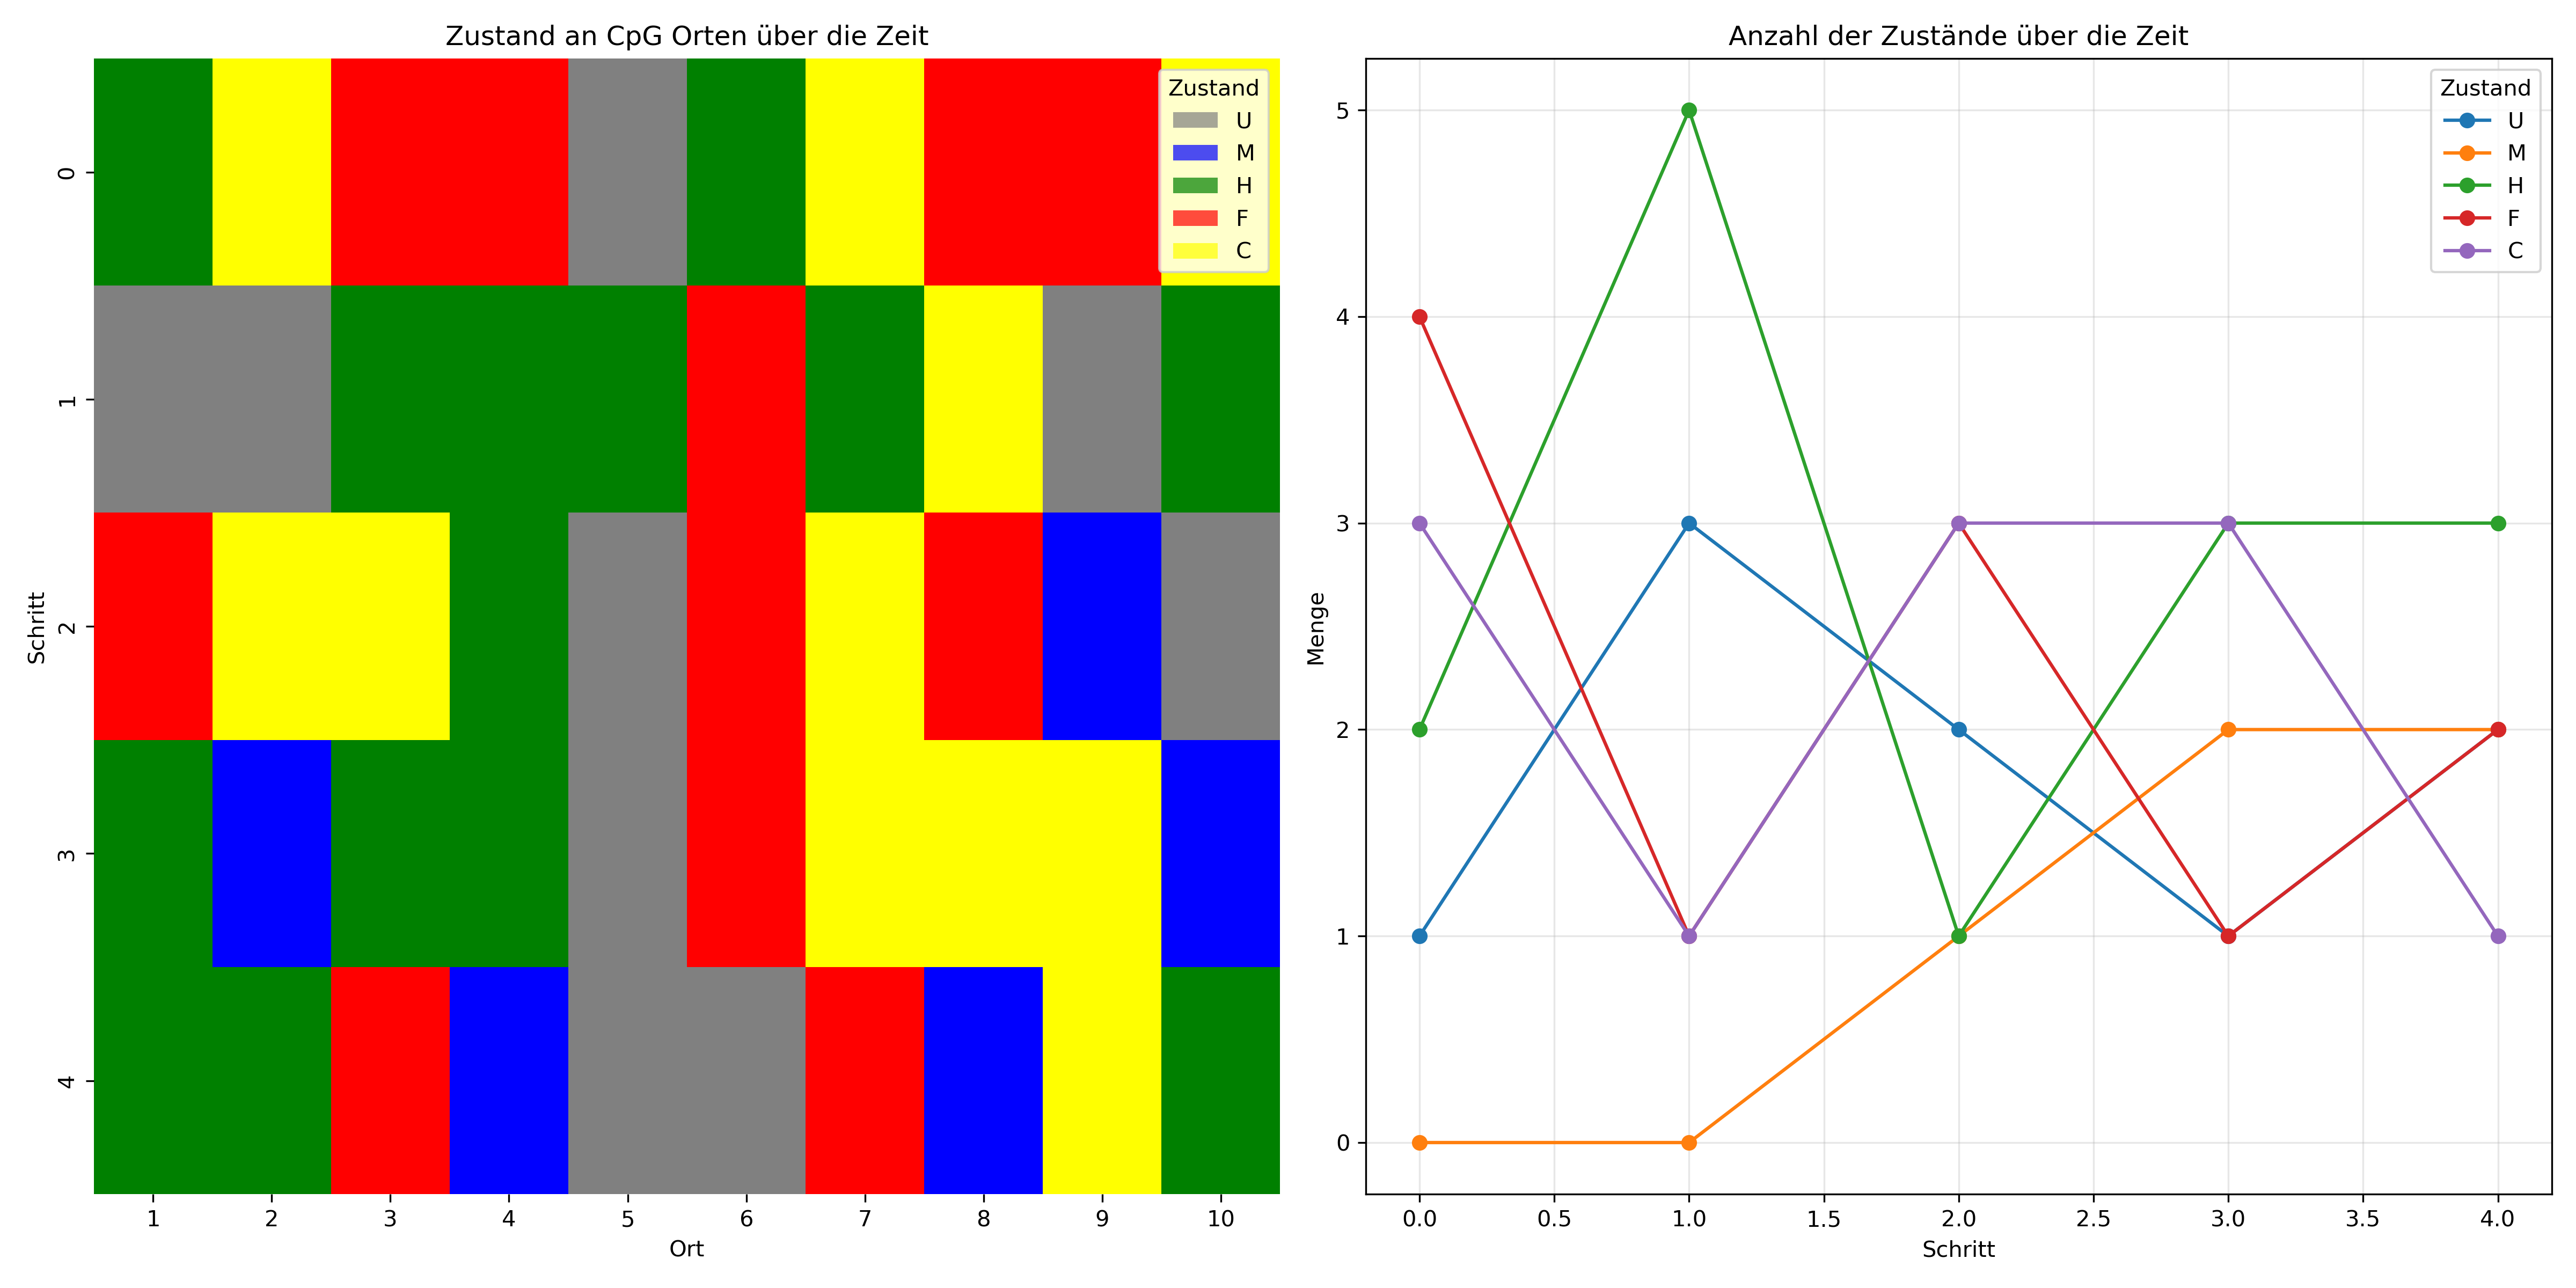
\includegraphics[width=0.9\textwidth]{images/cpg_states_plot.png}
  \caption{Visualisierung der CpG-Zust\"{a}nde \"{u}ber die Zeit. Links: Heatmap der Zust\"{a}nde an verschiedenen 
  CpG-Stellen \"{u}ber die Zeit (U: grau, M: blau, H: gr\"{u}n, F: rot, C: gelb). Rechts: Anzahl der CpG-Stellen in jedem Zustand \"{u}ber die Zeit.}
  \label{fig:cpg_states}
\end{figure}

\begin{figure}[htbp]
  \centering
  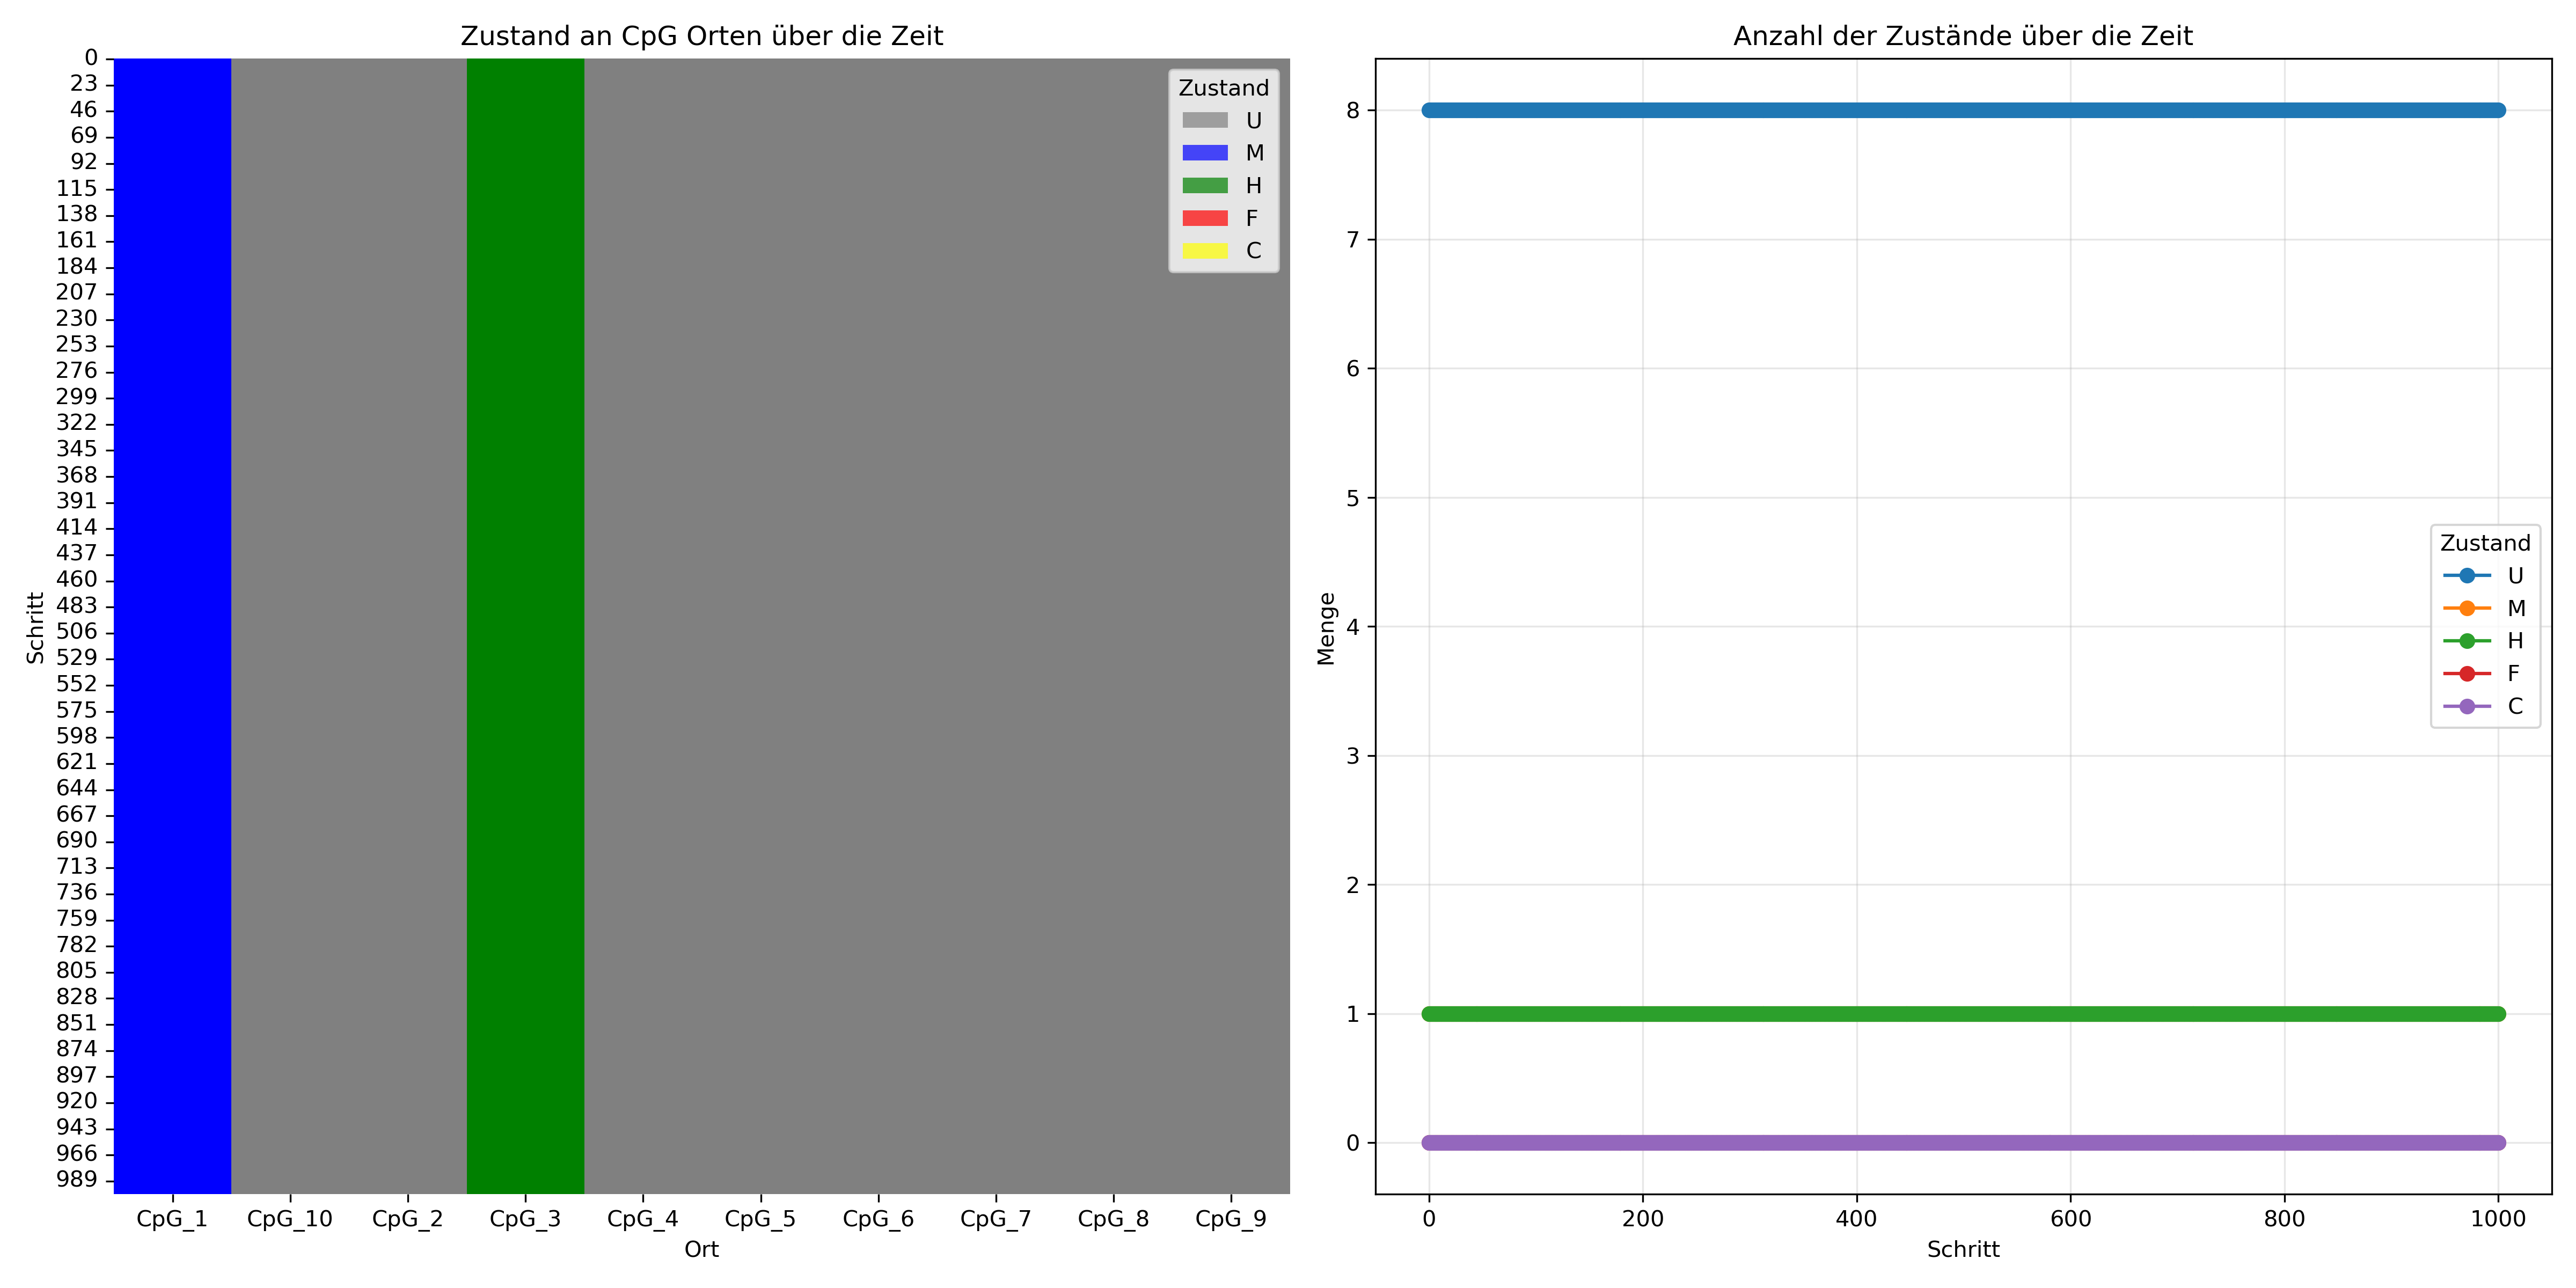
\includegraphics[width=0.9\textwidth]{images/cpg_states_plot_fu_1000.png}
  \caption{Visualisierung mit den Wahrscheinlichkeiten aus Fu et al. (2010) und 1000 Iterationen. \cite{fu-2010}}
  \label{fig:cpg_states_1000}
\end{figure}

\begin{figure}[htbp]
  \centering
  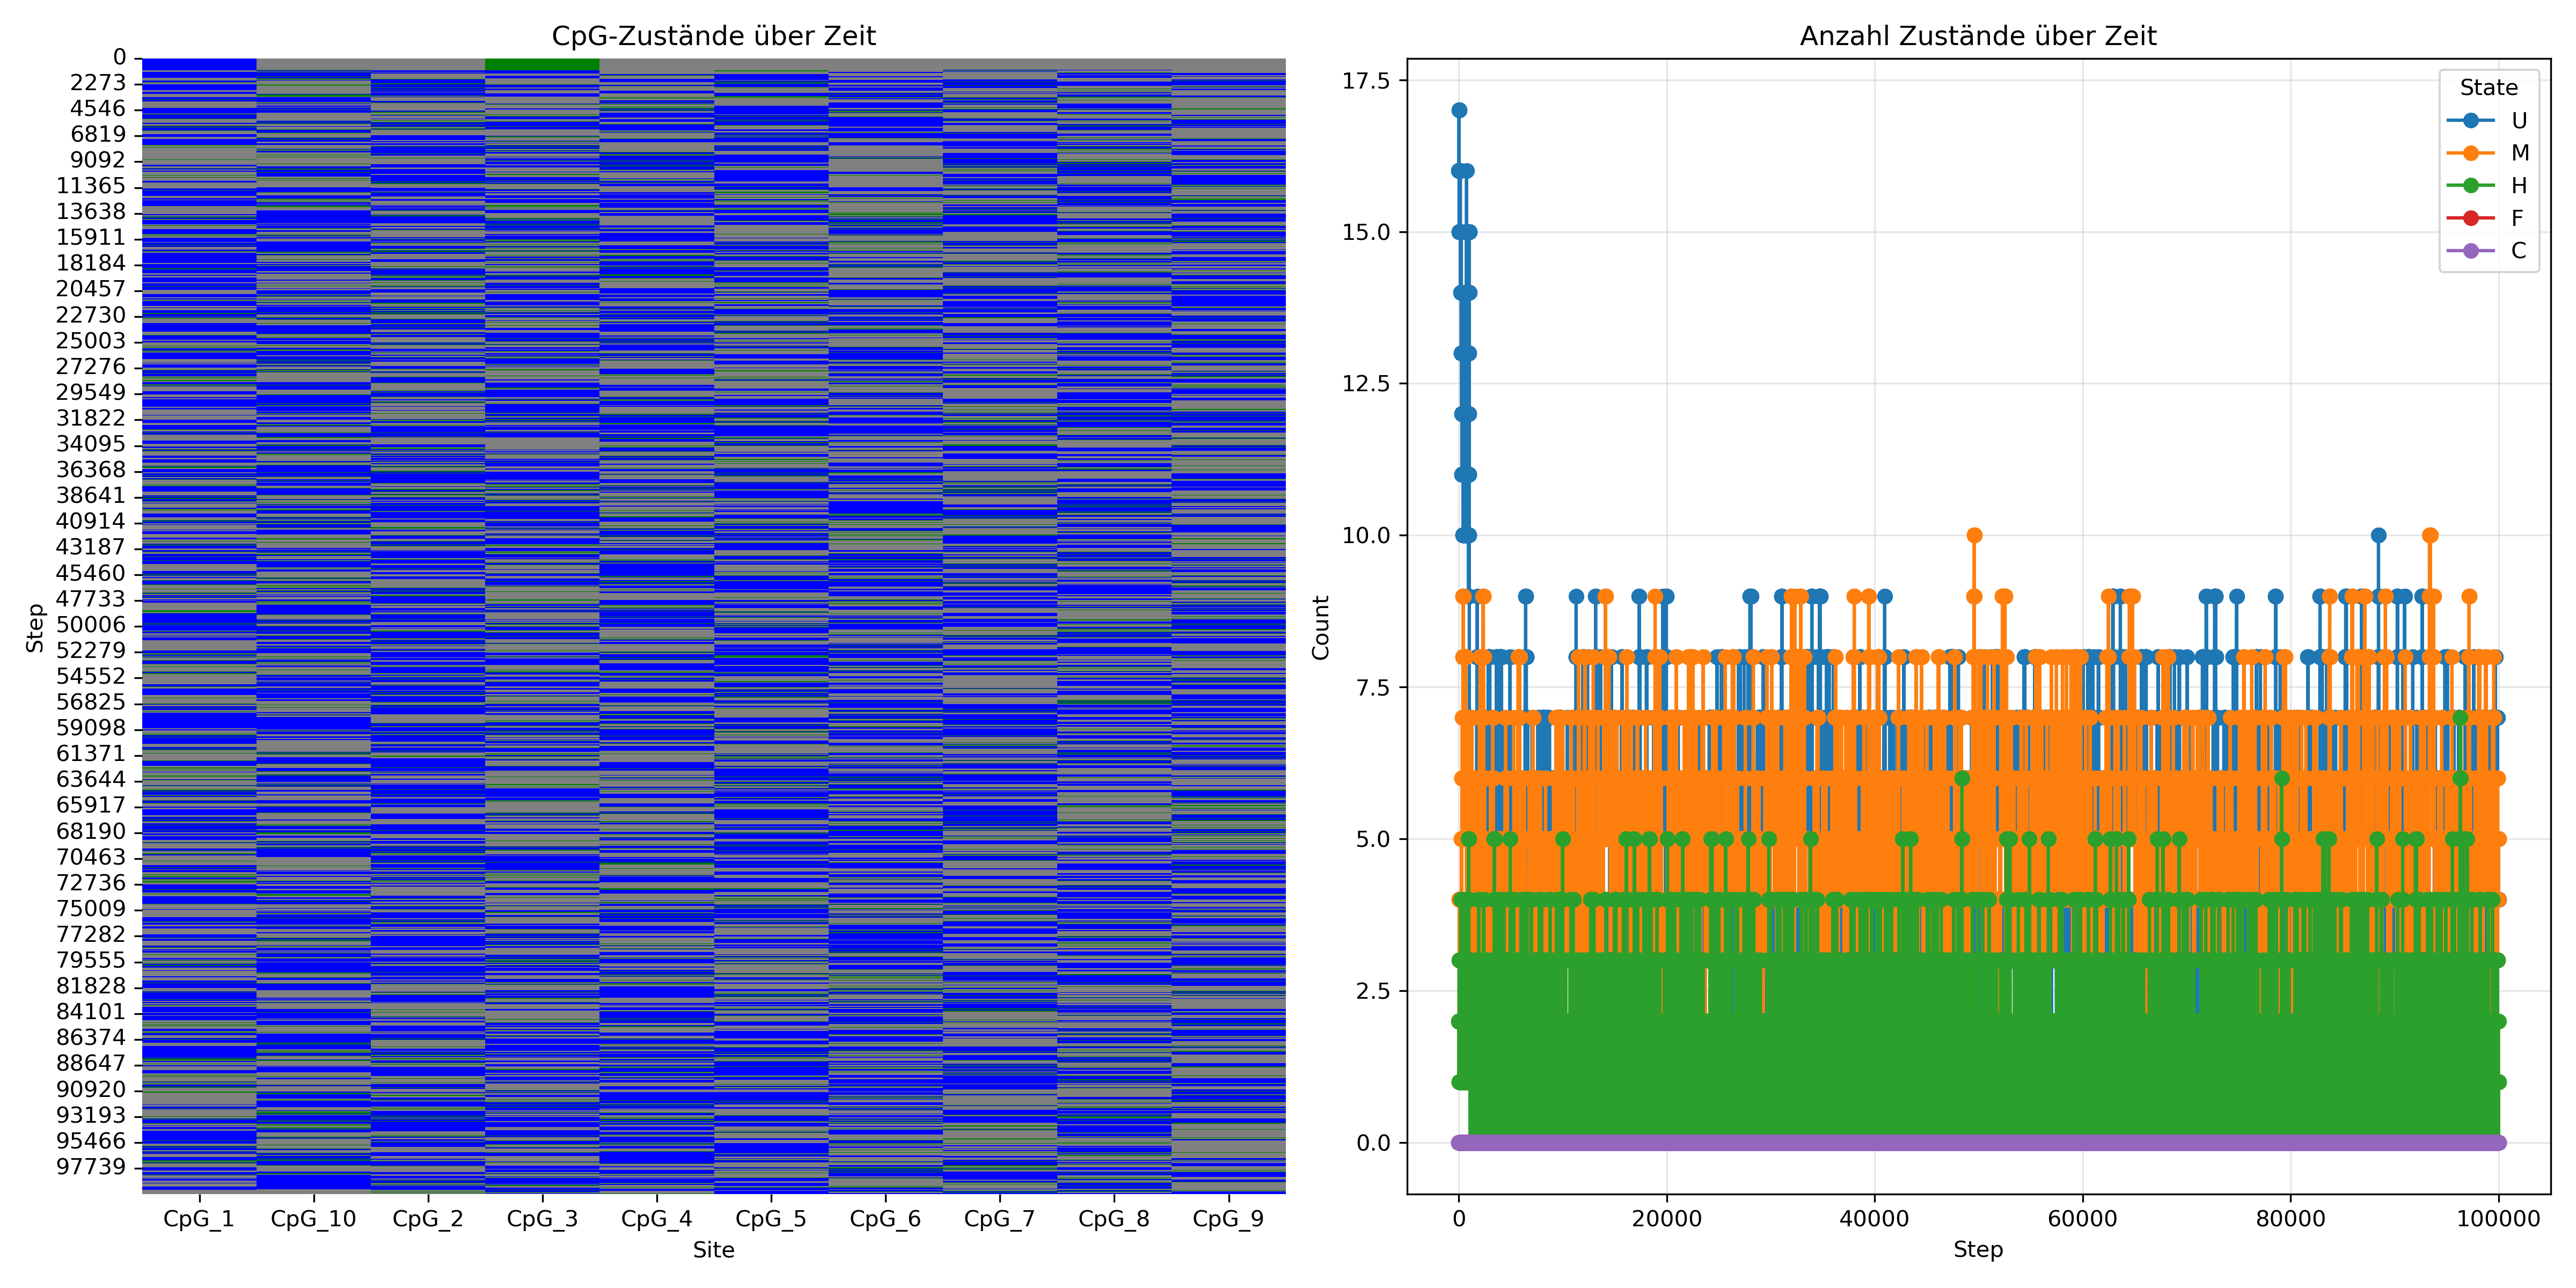
\includegraphics[width=0.9\textwidth]{images/cpg_states_plot_fu_100000.png}
  \caption{Visualisierung mit den Wahrscheinlichkeiten aus Fu et al. (2010) und 100000 Iterationen. \cite{fu-2010}}
  \label{fig:cpg_states_fu_100000}
\end{figure}

\begin{figure}[htbp]
\centering
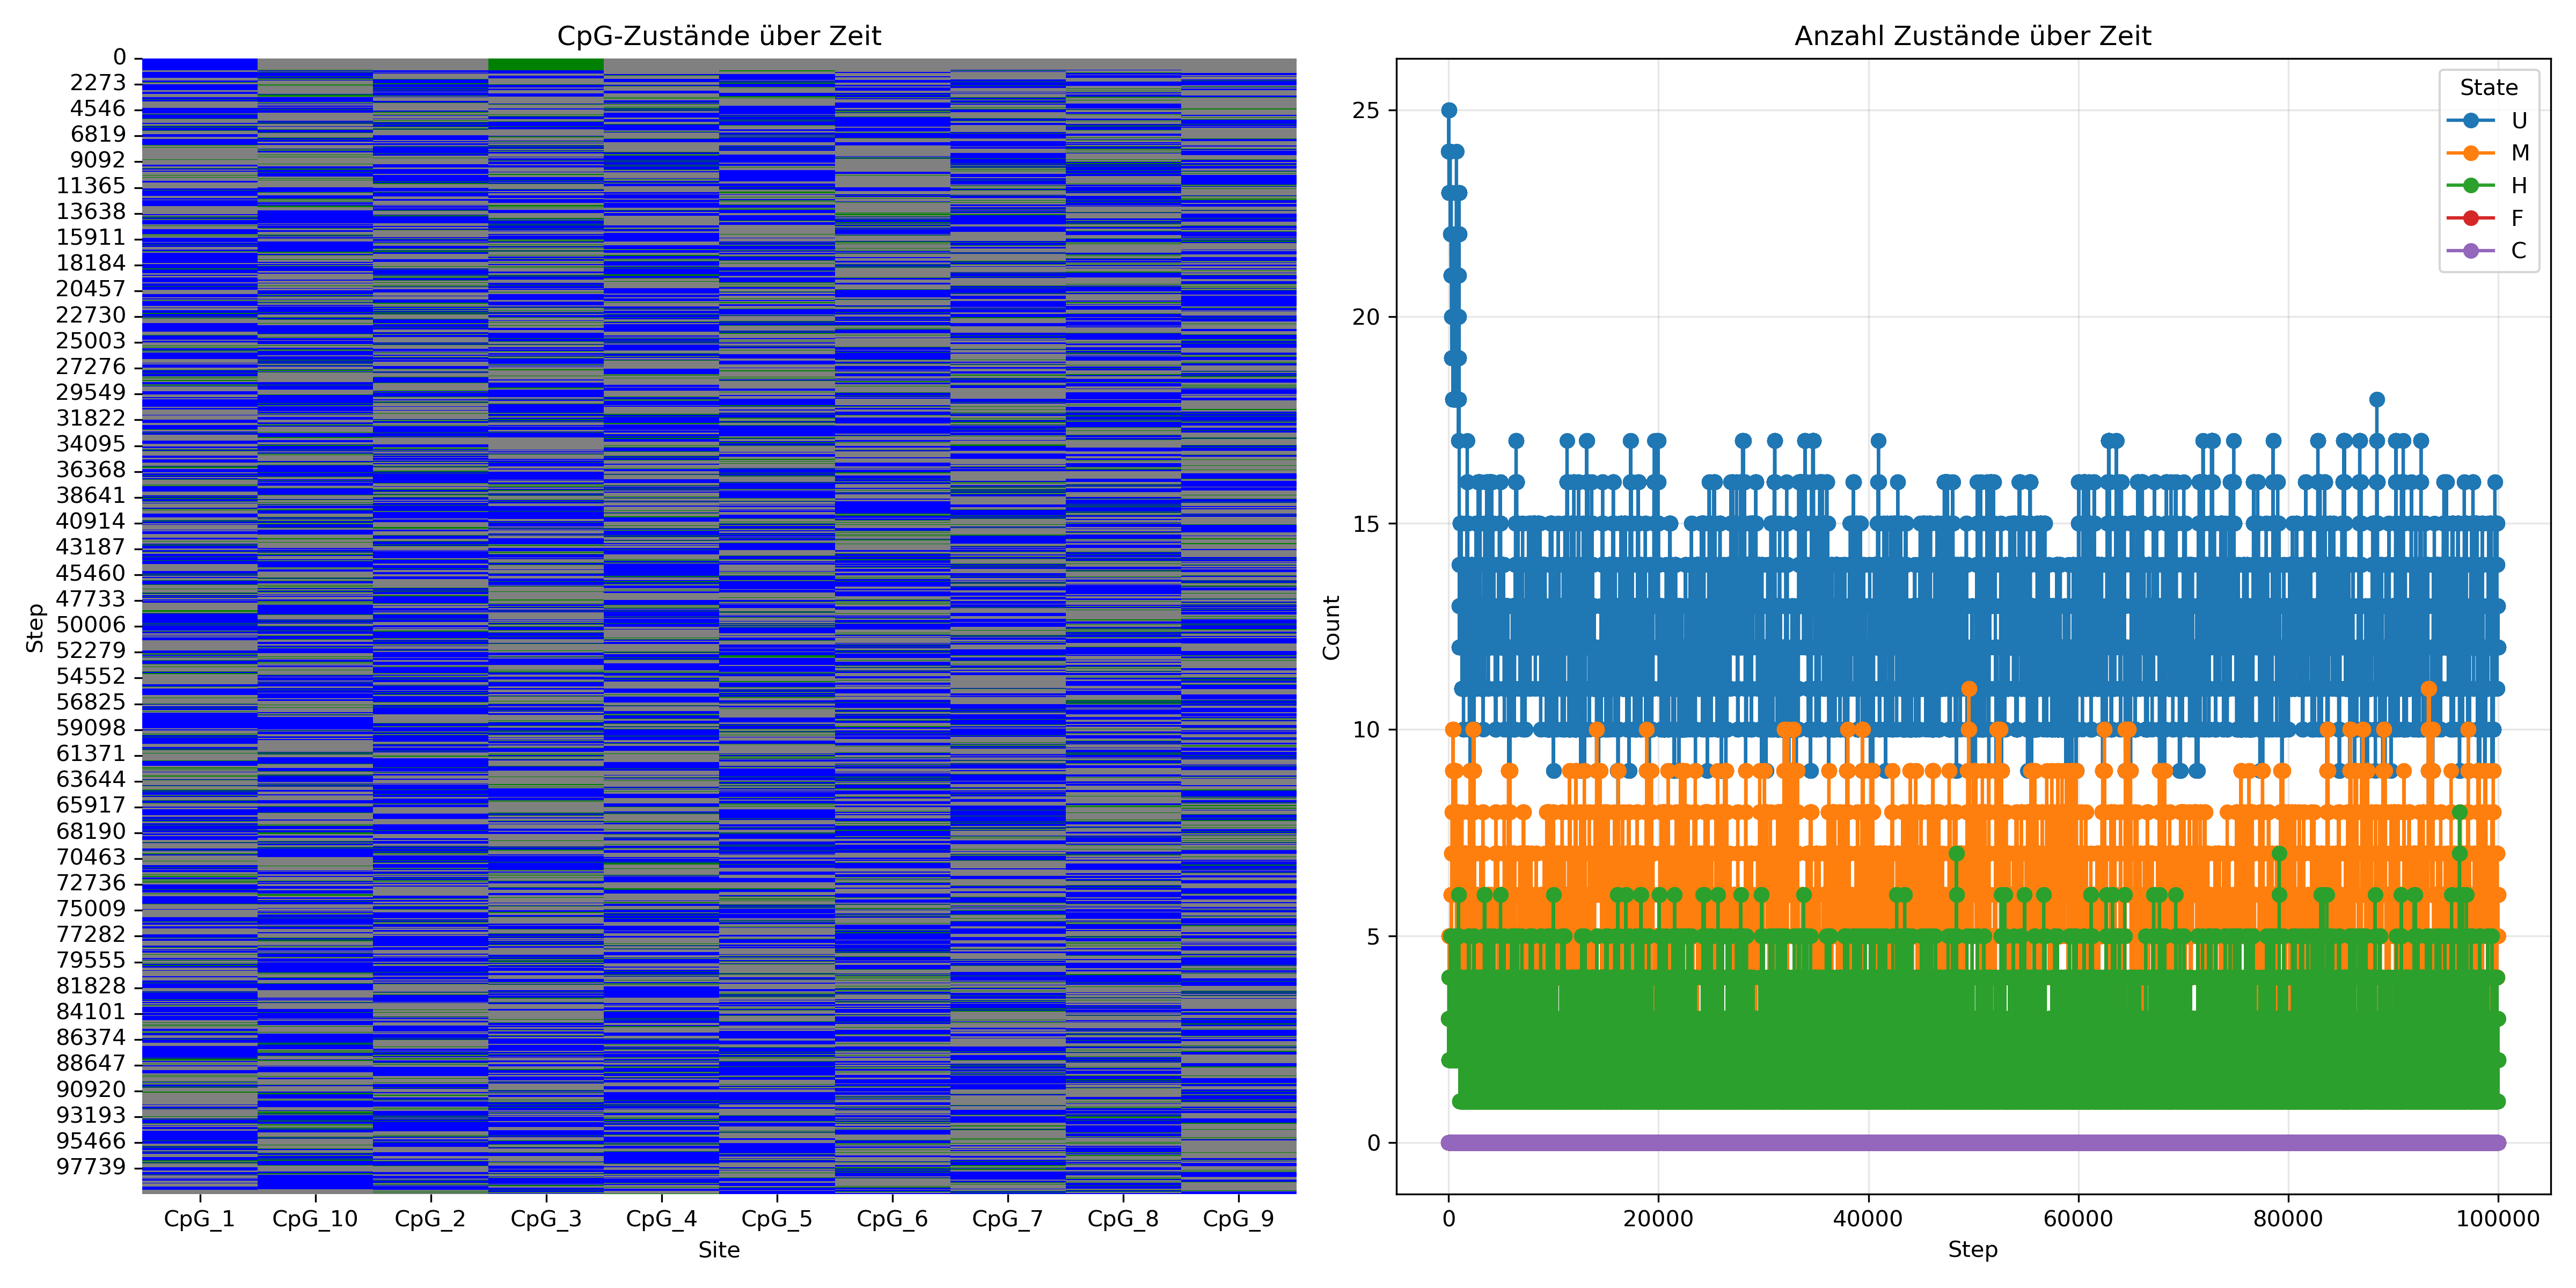
\includegraphics[width=0.9\textwidth]{images/cpg_states_plot_det.png}
\caption{Visualisierung des deterministischen Modells: links Heatmap der Zustände über die Zeit, rechts Häufigkeiten der Zustände.}
\label{fig:cpg_states_det}
\end{figure}

\begin{figure}[htbp]
\centering
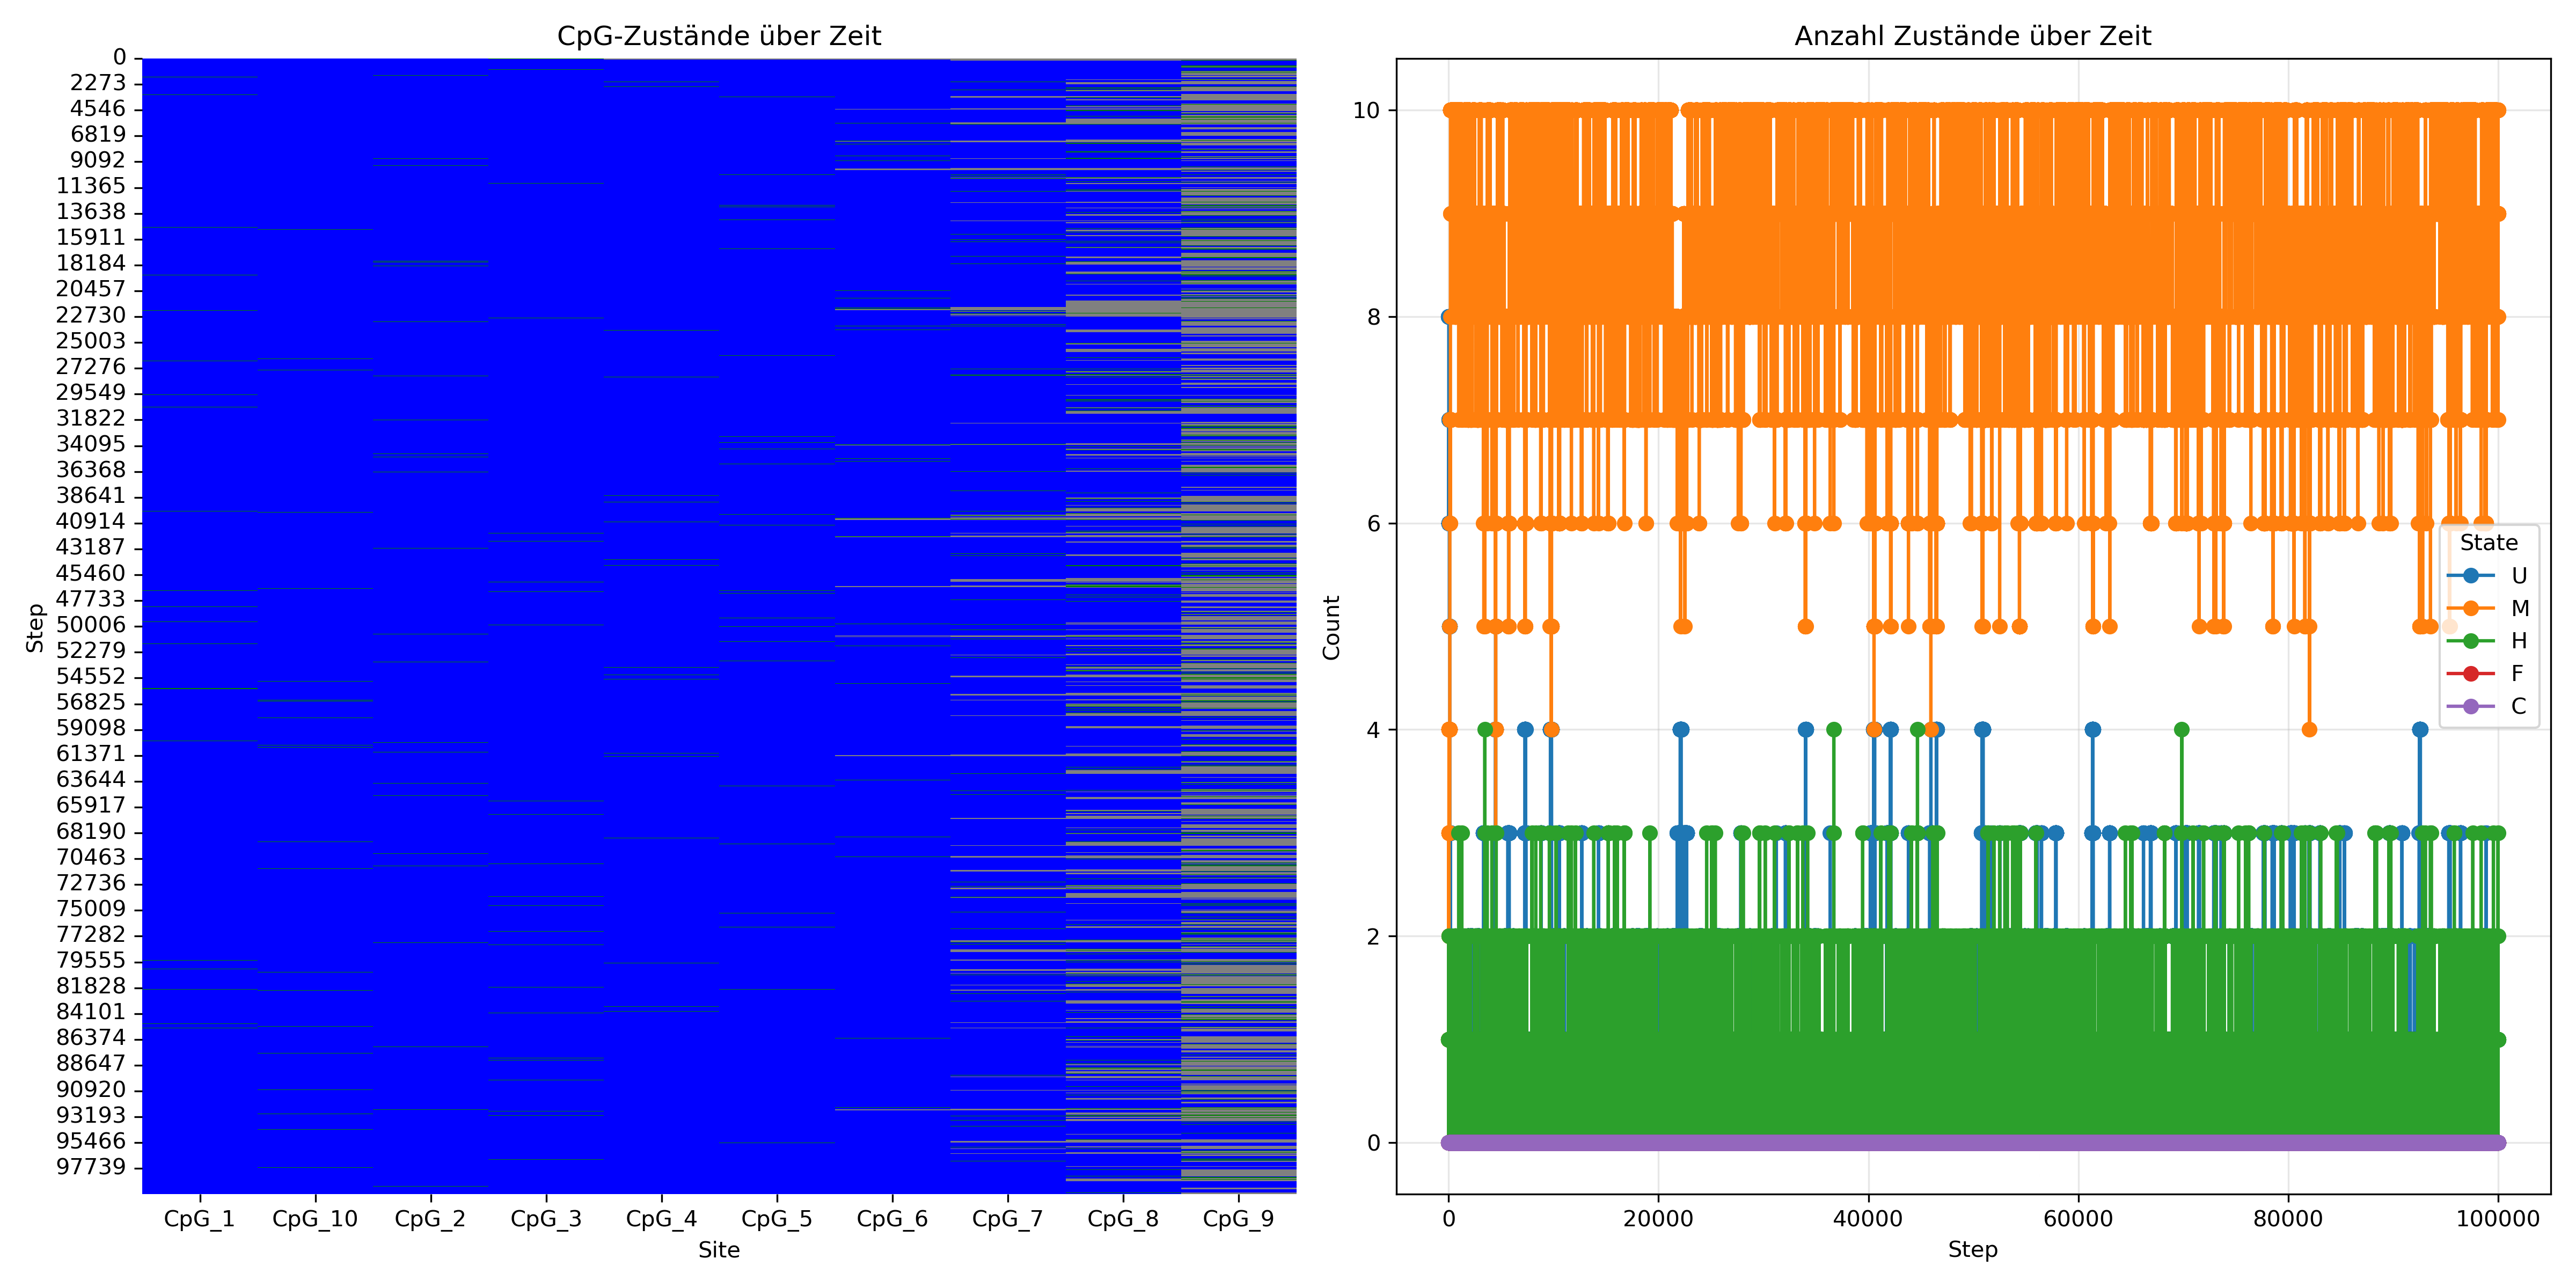
\includegraphics[width=0.9\textwidth]{images/cpg_states_plot_stoch.png}
\caption{Visualisierung des stochastischen Modells: links Heatmap der Zustände über die Zeit, rechts Häufigkeiten der Zustände.}
\label{fig:cpg_states_stoch}
\end{figure}


\begin{figure}[htbp]
  \centering
  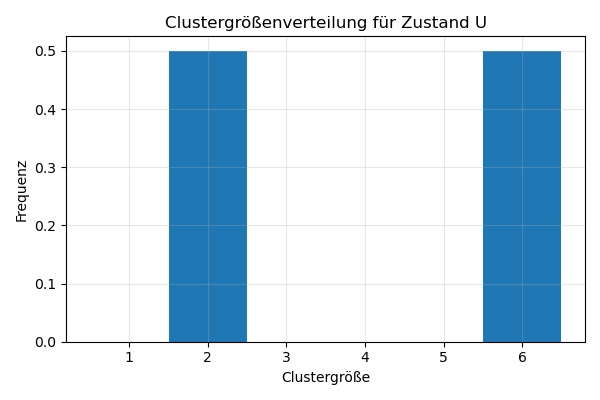
\includegraphics[width=0.9\textwidth]{images/Cluster_det.png}
  \caption{Clustergröße im deterministischen Modell}
  \label{fig:cpg_states_cluster_det}
  \end{figure}
\begin{figure}[htbp]
  \centering
  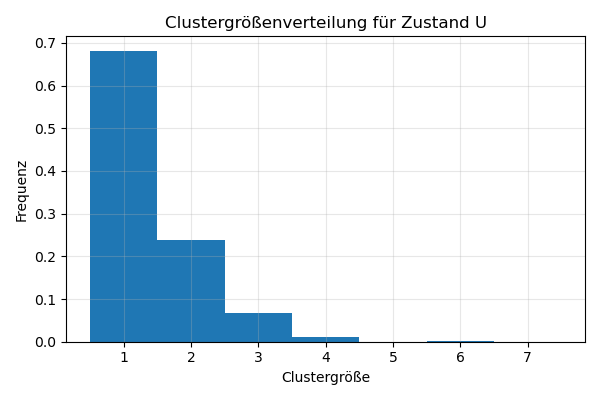
\includegraphics[width=0.9\textwidth]{images/Cluster_stoch.png}
  \caption{Clustergröße im stochastischen Modell}
  \label{fig:cpg_states_cluster_stoch}
  \end{figure}


\begin{figure} [htbp]
  \centering
  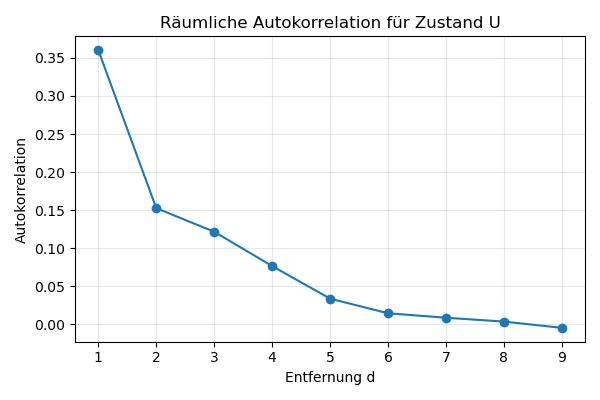
\includegraphics[width=0.9\textwidth]{images/Autokor_stoch.png}
  \caption{Autokorrelation im stochastischen Modell}
  \label{fig:cpg_states_auto_stoch}
  \end{figure}

\begin{figure}
  \centering
  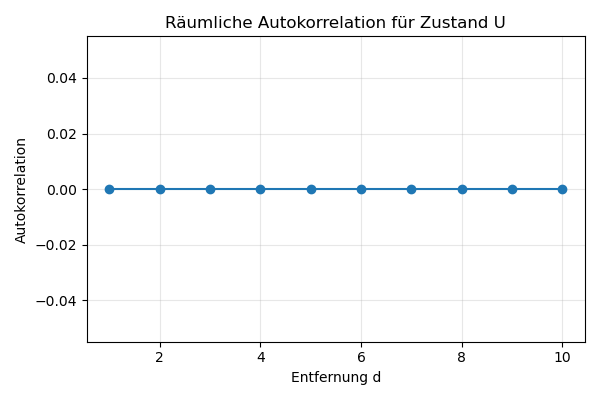
\includegraphics[width=0.9\textwidth]{images/Autokor_det.png}
  \caption{Autokorrelation im deterministischen Modell}
  \label{fig:cpg_states_auto_det}
\end{figure}


\begin{footnotesize}
\newpage
\bibliographystyle{unsrt}
\bibliography{own.bib}
\end{footnotesize}

\end{document}
